\documentclass[11pt]{article}

% "final" = non-anonymous camera-ready layout (course report).
\usepackage[final]{acl}

\usepackage{times}
\usepackage{latexsym}
\usepackage[T1]{fontenc}
\usepackage[utf8]{inputenc}
\usepackage{microtype}
\usepackage{inconsolata}
\usepackage{graphicx}
\usepackage{booktabs}
\usepackage{amsmath}
\usepackage{amssymb}
\usepackage{xcolor}

\newcommand{\qatrain}{\textsc{QA}\textsubscript{train}}
\newcommand{\qatest}{\textsc{QA}\textsubscript{test}}
\newcommand{\simtest}{\textsc{SimDom}\textsubscript{test}}
\newcommand{\hm}{\operatorname{HM}}
\newcommand{\todo}[1]{\textcolor{red}{[TODO: #1]}}

\title{Erased in English, Recalled in Russian:\\
Cross-Lingual Leakage of Embedding-Level Concept Erasure}

\author{Mary Arav \\
  Tel Aviv University \\
  \texttt{maryarav@mail.tau.ac.il} \\\And
  Ori Petel \\
  Tel Aviv University \\
  \texttt{oripetel@mail.tau.ac.il} \\\And
  Semyon Guretskiy \\
  Tel Aviv University \\
  \texttt{semyong@mail.tau.ac.il} \\}

\begin{document}
\maketitle

\begin{abstract}
Concept erasure aims to remove knowledge of a target concept from a language model's weights.
EMBER, a recent method, subtracts concept features from the input embeddings of concept-specific tokens and makes MLP-based erasure more robust to relearning, but its features and edited tokens come from English text.
We ask whether knowledge erased this way comes back when the model is asked about the concept in another language.
We erase 18 concepts from Gemma-2-2B-it with EMBER, an MLP-based method (SNMF) and their combination, tune every edit in English, and then ask held-out multiple-choice questions in English, German, Spanish, French and Russian.
Embedding-level erasure leaks: under EMBER, a concept retains on average 0.24 more of its knowledge in the other languages than in English, and 0.41 more in Russian, where the English edit reaches none of the concept's tokens.
SNMF erases all five languages about equally (leak $+0.01$), at the price of more collateral damage, and adding EMBER on top of SNMF strengthens English erasure but brings the leak back ($+0.16$).
The conclusions hold when unparseable answers are excluded.
Along the way we found a scoring artifact that inflated EMBER's efficacy at large edit strengths, replaced the paper's commercial judge with a validated local one, and found that fitting features on five languages jointly recovers almost no concept features at the default rank.
\end{abstract}

%=====================================================================
\section{Introduction}
%=====================================================================

Persistent concept erasure updates a model's parameters so that it can no longer produce knowledge about a target concept (e.g., \emph{Harry Potter}) while keeping its other abilities \citep{eldan2023harry,li2024wmdp,gurarieh2025precise}.
A recurring finding is that erasure is shallow: the knowledge can be recovered by fine-tuning on a little data, by rephrasing, or by changing the question format \citep{deeb2024unlearning,lynch2024eight,hong2025intrinsic,ye2025formindependent}.
\citet{suslik2026ember} argue that part of the problem is that erasure methods edit MLP layers and overlook the \emph{embedding} layer.
Their method, EMBER, factorizes the embeddings of concept-related tokens into sparse features and subtracts the concept features from a small set of concept tokens.
Combined with MLP-based methods, it improves erasure and makes it markedly more robust to relearning.

EMBER's features and edited tokens are found on English Wikipedia text.
An edit to the embedding rows of English tokens cannot change the representation of a German or Russian word that is spelled with other tokens, a limitation the EMBER paper itself names.
At the same time, multilingual models share much of their conceptual knowledge across languages in their middle layers \citep{wendler2024llamas,qi2023crosslingual}, and safety behavior trained in English often fails in other languages \citep{deng2024multilingual,yong2023lowresource}.
It is therefore unclear how much of an English embedding edit carries over to other languages, and whether this differs from erasure inside the MLPs.

We study two questions, following our proposal:
\textbf{(Q1) Cross-lingual leakage:} does erased knowledge re-emerge when the questions are translated, and does this differ between embedding-based and MLP-based erasure?
\textbf{(Q2) Multilingual extension:} can EMBER's feature search be run on multilingual data, and are the resulting concept features shared across languages?

We reproduce three erasure methods from the EMBER paper on Gemma-2-2B-it for all 18 of its concepts: EMBER alone, SNMF (an MLP-based method), and SNMF+EMBER.
Each edit is tuned in English with a validated local LLM judge, then evaluated, without re-tuning, on held-out multiple-choice questions translated into four languages.
Our findings (Figure~\ref{fig:retention}):
\begin{itemize}
\setlength\itemsep{1pt}
\item \textbf{EMBER leaks across languages.} Its erasure is weaker in every other language than in English (mean leak $+0.24$, 95\% CI $[+0.15,+0.32]$) and almost absent in Russian (retention 0.94).
\item \textbf{SNMF does not leak} ($+0.01$, $[-0.07,+0.09]$), but it also removes 30--40\% of knowledge about neighboring topics in every language.
\item \textbf{Adding EMBER to SNMF} gives the strongest English erasure but brings the leak back ($+0.16$), mostly into Russian.
\item \textbf{Mechanism.} The English EMBER edit touches none of the Russian concept words and almost none of the German ones, even though the embedding space contains a concept direction shared between English and Russian.
\item \textbf{Multilingual feature fitting} on five languages at the default rank found 0 embedding features for World War II, against 1 in English. We trace this to the rank and to mismatched data, and describe rebuilt data sets.
\item \textbf{Methodology.} A 4-token answer budget in the original multiple-choice scorer counted many correct answers as wrong under EMBER, inflating its efficacy at large edit strengths. We give corrected numbers and show that our leakage conclusions are robust to it.
\end{itemize}

\begin{figure}[t]
  \centering
  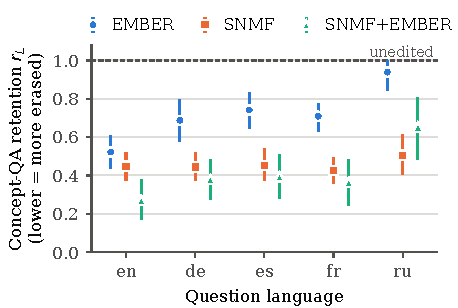
\includegraphics[width=\columnwidth]{figures/retention_by_language.pdf}
  \caption{Knowledge of the erased concept that remains in each question language (retention $r_L$, Eq.~\ref{eq:retention}; 1 = as before erasure, 0 = chance). Means over 18 concepts with 95\% bootstrap intervals. Every edit was tuned in English only.}
  \label{fig:retention}
\end{figure}

%=====================================================================
\section{Background and Related Work}
%=====================================================================

\paragraph{Concept erasure.}
Fine-tuning methods such as RMU \citep{li2024wmdp} and the Harry Potter unlearning of \citet{eldan2023harry} update many parameters with a forget objective.
Localize-then-edit methods instead find concept-related features and remove them: PISCES \citep{gurarieh2025precise} edits MLP parameters along features found with sparse autoencoders, and CRISP \citep{ashuach2026crisp} fine-tunes against such features.
SNMF, the MLP-based method we use, finds concept features in MLP activations with a semi-nonnegative matrix factorization \citep{ding2010convex,shafran2026constructing} and projects them out of the MLP weights, similar to directional ablation \citep{arditi2024refusal}.
Erased knowledge is often recoverable by relearning, adversarial prompting or a change of format \citep{deeb2024unlearning,lynch2024eight,hong2025intrinsic,ye2025formindependent}.

\paragraph{EMBER.}
Token embeddings encode factual and semantic knowledge \citep{geva2023dissecting}, including structure shared across languages \citep{wenyi2023hyperpolyglot}.
EMBER \citep{suslik2026ember} factorizes the embeddings $E_{\mathcal{V}^*}$ of the tokens that occur in a concept set $\mathcal{S}_C$ and a neutral set $\mathcal{S}_N$ (300 Wikipedia sentences each) as $E_{\mathcal{V}^*}^\top \approx ZY$, keeping the top 1\% of coefficients per feature.
Features whose coefficient mass is at least $\tau = 2$ times larger on concept-only tokens than on neutral tokens, and that an LLM judges to be the concept, form $\mathcal{F}_C$.
Each concept token $t$ with a nonzero coefficient on some feature in $\mathcal{F}_C$ is edited as
\begin{equation}
  \mathbf{e}_t \leftarrow \mathbf{e}_t - \delta \textstyle\sum_{i \in \mathcal{F}_C} Y_{i,t}\,\mathbf{z}_i .
  \label{eq:ember}
\end{equation}
On Gemma this edits only 31--86 tokens per concept.
The paper names language coverage as a limitation and suggests multilingual concept sets as future work; we test both.

\paragraph{Cross-lingual knowledge and unlearning.}
Multilingual LMs process many languages through a shared, English-leaning concept space in their middle layers \citep{wendler2024llamas}, with language-specific neurons concentrated in the first and last layers \citep{tang2024languagespecific}.
Facts are not equally consistent across languages, and edits made in English transfer mainly to languages that are consistent with it \citep{qi2023crosslingual,wang2024crosslingualediting}.
Safety training in English transfers poorly to low-resource languages \citep{deng2024multilingual,yong2023lowresource}.
For unlearning specifically, \citet{choi2024crosslingual} show that unlearning in one language does not reliably carry over to others, \citet{lu2025learn} find that English-only unlearning fails to remove misinformation planted in other languages, and \citet{farashah2026amnesia} study how unlearning transfers between languages.
These works use fine-tuning-based unlearning or knowledge editing.
To our knowledge, no prior work studies embedding-level erasure across languages, where the edit is tied to specific vocabulary rows and, by construction, cannot reach tokens of another script.

%=====================================================================
\section{Method}
%=====================================================================

\subsection{Erasure methods and data}
We use Gemma-2-2B-it \citep{gemma2024gemma2} in bfloat16 with greedy decoding, the 18 concepts of \citet{suslik2026ember}, and their released features (rank 100, seed 42).\footnote{For World War II, the released features match the paper's count (1 embedding and 15 MLP features).}
\textbf{EMBER} applies Eq.~\ref{eq:ember} with $\delta \in \{0.5,1,2,5,10,50,100,200\}$.
\textbf{SNMF} removes each concept MLP feature $\mathbf{f}$ (unit norm, restricted to its neuron support) from the MLP output weights, $W \leftarrow W - \delta_{\text{out}}\,\mathbf{f}\mathbf{f}^\top W$, and similarly from the input weights with $\delta_{\text{in}}$.
Its grid has $\delta_{\text{in}},\delta_{\text{out}} \in \{1,4,7,10\}$, input layers 0--8, 0--12 or 0--25, and output layers 0--8, 9--17 or 13--25: 144 cells.
\textbf{SNMF+EMBER} fixes the concept's selected EMBER $\delta$ and searches the SNMF grid again on top of it, as in the paper.

Each concept has 50 multiple-choice questions for selection (\qatrain) and 50 held-out ones (\qatest), plus 50+50 on a similar but distinct domain (\textsc{SimDom}; e.g., other fantasy novels for Harry Potter).
General ability is measured with MMLU \citep{hendrycks2021mmlu} and coherence with AlpacaEval prompts \citep{taori2023alpaca}, scored by an LLM judge for instruction following and fluency (0--2 each).

\subsection{Selection metric}
All scores are fractions of the unedited model's score, corrected for the 0.25 chance level of four-option questions:
\begin{equation}
  \phi(a; a_0) = \operatorname{clip}\!\left(\tfrac{a - 0.25}{a_0 - 0.25},\,0,\,1\right),
\end{equation}
where $a$ is the edited and $a_0$ the unedited accuracy.
Efficacy is $1 - \phi(\text{QA})$, specificity is $\hm(\phi(\text{MMLU}), \phi(\textsc{SimDom}))$, and coherence is the harmonic mean ($\hm$) of the two judge scores, each as a fraction of the unedited model's score, capped at 1.
The final selection score is $\hm(\text{efficacy}, \text{specificity}, \text{coherence})$.
Following the paper, EMBER candidates must keep MMLU and both judge fractions at $\geq 0.9$; SNMF has no judge gate.

\subsection{Selection with a local judge}
The paper's judge is Gemini.
A full search over 18 concepts needs about 43{,}000 judge calls, so we replaced it with Qwen2.5-32B-Instruct \citep{qwen2024qwen25}, run locally with 4-bit NF4 quantization \citep{dettmers2023qlora}.
It is free to run and comes from a different model family than the model being erased, so it stays an independent measuring instrument \citep[cf.][]{zheng2023judging}.
We validated it by re-judging the 150 completions Gemini had already scored, item by item, with the same prompts.
Its mean scores differ from Gemini's by $-0.07$ (instruction) and $+0.04$ (fluency), inside our $\pm 0.15$ acceptance band.
Qwen2.5-14B ($+0.20$ on fluency) and Gemma-4-12B ($+0.37$, and from the same family as the erased model) failed (Appendix~\ref{app:judge}).
Item-level fluency agreement is only 64\%, so we use the judge only through means over many items.

Selection has two passes.
Pass~1 ranks all candidates by the judge-free $\hm(\text{efficacy},\text{specificity})$.
Pass~2 judges the first 50 AlpacaEval answers of the top three candidates and picks the highest full score.
For EMBER, re-deriving this choice from earlier full-grid judging (8 values of $\delta$, 150 answers) reproduced 10 of 12 picks; the other two were near-ties.
For one concept (Ancient Rome) all three shortlisted SNMF cells produced degenerate text (``Roman Roman Roman \ldots''), which multiple-choice scores cannot see.
We skipped cells in which more than 10\% of answers loop (Appendix~\ref{app:loop}).

\subsection{Cross-lingual evaluation}
\label{sec:xl}
We machine-translated \qatest{} and \simtest{} into German (de), Spanish (es), French (fr) and Russian (ru).\todo{name the translation tool}
We repaired the translations: 19 questions where two options collapsed into the same string, one with a hallucinated fifth option, 30 whitespace defects and one encoding error (Appendix~\ref{app:data}).
The whole prompt is in the target language, and only the answer letters stay A--D.
The option order is seeded per question, so a question has the same correct letter in every language and the model's letter preferences cannot appear as a language effect.
Each edit is applied once, exactly as selected in English, and never re-tuned.
For each concept, method and language $L$ we compute the retention and the leak
\begin{equation}
  r_L = \phi\big(\mathrm{acc}_L;\ \mathrm{acc}^{\text{unedited}}_L\big), \qquad \Delta_L = r_L - r_{\text{en}},
  \label{eq:retention}
\end{equation}
so the denominator is the unedited model's accuracy in the same language, and $\Delta_L > 0$ means the concept survives better in $L$ than in English.
We drop a (concept, language) pair when the unedited model scores below 0.40 there: 2 of 90 pairs (Harry Potter and Valentine's Day in Russian).
Collateral damage is measured with $\phi$ on \simtest{} in every language and with the 1000-question English MMLU test split.
Each concept is one unit: we average over concepts and report 95\% bootstrap intervals over concepts (10{,}000 resamples), because a single cell (50 questions) has a standard error of about 0.3 on $\Delta$.
All 54 edits reproduced their English selection scores exactly when re-applied.

%=====================================================================
\section{Results}
%=====================================================================

\subsection{Erasure in English}

\begin{table}[t]
\centering\small
\setlength{\tabcolsep}{4pt}
\begin{tabular}{@{}lcccc@{}}
\toprule
Method & Effic. & Spec. & Coher. & Score \\
\midrule
EMBER       & 0.52 & \textbf{0.97} & \textbf{0.99} & 0.74 \\
SNMF        & 0.72 & 0.85 & 0.96 & 0.82 \\
SNMF+EMBER  & \textbf{0.88} & 0.91 & 0.96 & \textbf{0.91} \\
\midrule
\multicolumn{5}{@{}l}{\emph{held-out English retention $r_{\text{en}}$ (\qatest, lower is better)}} \\
\multicolumn{5}{@{}l}{EMBER 0.52 \quad SNMF 0.45 \quad SNMF+EMBER \textbf{0.27}} \\
\bottomrule
\end{tabular}
\caption{English erasure of the selected edits, mean over 18 concepts. The top block shows selection scores on \qatrain{}, which are optimistic because the edits were chosen on these items. EMBER and SNMF+EMBER efficacy is also inflated by the scoring artifact of \S\ref{sec:artifact}.}
\label{tab:english}
\end{table}

Table~\ref{tab:english} shows the selected edits.
EMBER barely harms the model but removes only about half of the concept, SNMF erases more at a higher cost, and the combination scores best on 17 of 18 concepts, consistent with \citet{suslik2026ember}.
The held-out English retention follows the same order.
Per-concept results are in Appendix~\ref{app:concepts}.

\subsection{Cross-lingual leakage}

\begin{table*}[t]
\centering\small
\resizebox{\textwidth}{!}{%
\begin{tabular}{@{}lccc@{}}
\toprule
 & EMBER & SNMF & SNMF+EMBER \\
\midrule
English \qatest{} accuracy (unedited 0.73) & 0.50 & 0.47 & \textbf{0.38} \\
Retention $r_L$: en / de / es / fr / ru & 0.52 / 0.69 / 0.74 / 0.71 / 0.94 & 0.45 / 0.44 / 0.45 / 0.43 / 0.51 & 0.27 / 0.38 / 0.39 / 0.36 / 0.65 \\
\midrule
Leak $\Delta_{\text{de}}$ & $+0.17$ [$+0.07$, $+0.27$] & $-0.00$ [$-0.08$, $+0.07$] & $+0.11$ [$-0.01$, $+0.23$] \\
Leak $\Delta_{\text{es}}$ & $+0.22$ [$+0.12$, $+0.33$] & $+0.00$ [$-0.10$, $+0.12$] & $+0.12$ [$+0.03$, $+0.23$] \\
Leak $\Delta_{\text{fr}}$ & $+0.19$ [$+0.09$, $+0.29$] & $-0.02$ [$-0.12$, $+0.08$] & $+0.09$ [$+0.00$, $+0.19$] \\
Leak $\Delta_{\text{ru}}$ & $+0.41$ [$+0.28$, $+0.52$] & $+0.05$ [$-0.06$, $+0.15$] & $+0.37$ [$+0.20$, $+0.54$] \\
\textbf{Mean leak over de/es/fr/ru} & $\mathbf{+0.24}$ [$+0.15$, $+0.32$] & $\mathbf{+0.01}$ [$-0.07$, $+0.09$] & $\mathbf{+0.16}$ [$+0.07$, $+0.26$] \\
Concepts with mean leak $> 0$ & 16 / 18 & 9 / 18 & 14 / 18 \\
Mean leak, unparseable answers dropped & $+0.19$ [$+0.12$, $+0.27$] & $+0.01$ [$-0.07$, $+0.09$] & $+0.11$ [$+0.02$, $+0.20$] \\
\midrule
\simtest{} retention: en / de / es / fr / ru & 0.96 / 0.98 / 0.98 / 0.98 / 1.00 & 0.73 / 0.62 / 0.65 / 0.68 / 0.59 & 0.81 / 0.69 / 0.75 / 0.77 / 0.76 \\
English MMLU, 1000 questions (unedited 0.553) & \textbf{0.548} & 0.506 & 0.511 \\
Unparseable answers on \qatest: en / mean of others & 0.09 / 0.05 & 0.00 / 0.00 & 0.16 / 0.08 \\
\bottomrule
\end{tabular}
}
\caption{Cross-lingual evaluation of English-tuned edits, means over 18 concepts (16 for Russian) with 95\% bootstrap intervals over concepts. Retention $r_L$ and leak $\Delta_L = r_L - r_{\text{en}}$ are defined in Eq.~\ref{eq:retention}. The mean leak first averages each concept over its reliable languages. Lower \simtest{} retention and MMLU mean more collateral damage.}
\label{tab:crossling}
\end{table*}

Table~\ref{tab:crossling} and Figure~\ref{fig:retention} give the answer to Q1.

\paragraph{The embedding edit leaks.}
Under EMBER, every non-English language retains more of the concept than English, with intervals that exclude zero for all four languages.
16 of 18 concepts leak on average.
Russian is the extreme: retention 0.94, close to the unedited model.
Its retention is higher than the mean of German, Spanish and French in 15 of 16 concepts (by $+0.22$, $[+0.13,+0.31]$).

\paragraph{The MLP edit erases evenly but broadly.}
SNMF has no detectable leak in any language, and about half the concepts go each way.
It is also much less specific: it removes 27--41\% of similar-domain knowledge (EMBER: 0--4\%) and lowers English MMLU from 0.553 to 0.506.
Part of SNMF's evenness therefore comes from a broader edit.
The 50-question MMLU set used for selection (standard error $\approx 0.07$) cannot detect a 0.05 drop, so the selection procedure could not prevent this.

\paragraph{The combination leaks again.}
SNMF+EMBER erases English the most ($r_{\text{en}}=0.27$), but adding the embedding edit on top of SNMF brings the leak back, mainly in Russian ($+0.37$).
Paired by concept, EMBER leaks more than SNMF by $+0.23$ ($[+0.14,+0.32]$, $t=4.9$), and SNMF+EMBER more than SNMF by $+0.15$ ($[+0.04,+0.27]$).
EMBER and SNMF+EMBER are not clearly different ($+0.08$, $[-0.01,+0.17]$).
An earlier run of the same experiment, on 8 concepts with Gemini-based selection and a different option order, found the same ordering (leaks of $+0.25$, $+0.10$ and $+0.22$).

\subsection{A scoring artifact and its effect}
\label{sec:artifact}

\begin{figure}[t]
  \centering
  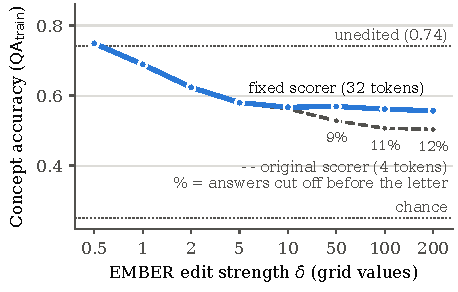
\includegraphics[width=\columnwidth]{figures/ember_rescore.pdf}
  \caption{EMBER's concept accuracy on \qatrain{} for each grid value of $\delta$, mean over 18 concepts. The original scorer allows 4 new tokens and so cuts off answers such as ``The answer is **C**'' before the letter, counting them as wrong. With 32 tokens, accuracy stops falling after $\delta = 10$.}
  \label{fig:artifact}
\end{figure}

The paper's multiple-choice scorer generates 4 new tokens and reads the first capital letter.
The unedited model answers with a bare letter, but under a strong embedding edit Gemma often answers in a sentence (``The answer is **C**'', ``La respuesta correcta es \ldots'').
The 4-token cut ends before the letter, and the answer is counted as wrong, which looks like successful erasure.
About 90\% of the unparseable answers we inspected were such cut-off phrases rather than broken text.
The effect is specific to questions about the erased concept: at most 1\% on \textsc{SimDom} and MMLU.

We re-scored the whole EMBER grid with a 32-token budget and a stricter parser.
Greedy decoding makes this a controlled comparison: the first 4 tokens of the new outputs reproduced the old outputs for 17 of 18 concepts.\footnote{For the 18th (Pornography) the control failed; its selected $\delta$ had no unparseable answers.}
Figure~\ref{fig:artifact} shows the result.
With correct scoring, EMBER's concept accuracy stops falling at $\delta \approx 10$; the further decrease at $\delta \geq 50$ was the artifact.
At the selected edits, mean \qatrain{} accuracy rises from 0.49 to 0.54 and efficacy drops from 0.52 to 0.42 (Uranium: 0.82 to 0.31), and for 8 of 18 concepts the selected $\delta$ changes or a new candidate has to be judged.
SNMF+EMBER is affected more (15\% unparseable answers at its selected edits); SNMF's selected edits are not affected.
Re-selecting these edits requires new judging and is in progress, so the EMBER and SNMF+EMBER numbers above should be read as using the original scorer.

Does the artifact explain the leak?
Unparseable answers are most frequent in English (Table~\ref{tab:crossling}), which lowers $r_{\text{en}}$ and inflates $\Delta$.
Dropping them from both the edited and the unedited model's scores lowers EMBER's mean leak from $+0.24$ to $+0.19$ and SNMF+EMBER's from $+0.16$ to $+0.11$, and both intervals still exclude zero (Table~\ref{tab:crossling}).
The leak into Russian, where unparseable answers are rare (1--2\%), stays large ($+0.31$ and $+0.27$).
The direction of every conclusion in this section is therefore robust to the artifact, while its exact size will change with re-selection.

\subsection{Why EMBER leaks}
\label{sec:mechanism}

\paragraph{The edit does not reach foreign tokens.}
Gemma splits most Russian and German concept words into several pieces: only 4 of 50 Russian and 8 of 50 German words for Gun and Heroin are single tokens.
Using lists of about 25 concept words per concept and language, we measured which words an English-fitted EMBER edit actually touches, for five concepts (Gun, Heroin, Gambling, Ancient Rome, World War II), three seeds and the top three features.
It edits at least one piece of 45\% of the English concept words, but of 0\% of the Russian and German ones and 3\% and 1\% of the Spanish and French ones.
Since EMBER changes only whole vocabulary rows, a Russian question passes through the network almost unedited.
This matches the language ordering in Figure~\ref{fig:retention}: Latin-script languages share some surface forms with English (names, cognates), and Russian shares none.
In the earlier 8-concept run, concepts whose translated questions shared fewer words with English leaked more under EMBER ($r = -0.68$) and SNMF+EMBER ($r = -0.91$), but not under SNMF ($r = +0.20$).

\paragraph{A shared concept direction exists.}
The missing transfer is not because the concept lacks a cross-lingual representation in the embedding matrix.
For each of the five concepts we built a direction from about 25 Russian concept words (mean of their piece embeddings minus the mean of ordinary Russian words).
This direction ranks the English words of the same concept above English words of the other four concepts with AUC 0.99 (Gun), 0.95 (Heroin), 0.95 (Gambling) and 0.86 (Ancient Rome), even though no word shares a surface form.
It fails for World War II (0.41), whose Russian words are mostly transliterated names.
Yet only 1--7\% of the Russian direction lies in the subspace of EMBER's English features.
The shared structure exists, but the English-fitted features are too narrow to express it.

\subsection{Toward multilingual EMBER (Q2)}
\label{sec:multi}

\paragraph{Joint fitting, embedding level.}
We refit EMBER's factorization with concept and neutral sentences from English plus Russian, or English plus all four languages, taken from the corresponding Wikipedia articles (5 concepts, 3 seeds).
Adding languages did not separate Russian concept words better (AUC against other concepts' words 0.54 to 0.53) and made English worse (0.74 to 0.67).
The joint edit reaches more foreign concept words (Spanish: 3\% to 18\%), but by editing about four times as many tokens (108 to 419) with a weaker per-token edit.

\paragraph{Full pipeline, World War II.}
Running the complete feature search (both factorizations and the same LLM feature filter) on 3{,}000 sentences in five languages kept \textbf{0} embedding and \textbf{2} MLP features, against 1 and 15 in English.
The surviving candidates are cross-lingual but generic: ``armed forces'' (\emph{military, militares, militaire}), ``attack'', past-tense verbs, and ``however''.
No embedding feature for Hitler, Nazi or 1939--1945 exists.
We identify three causes.
(1) Rank 100 was tuned for 600 English sentences; with five languages, the factorization spends its features on structure shared by all of them.
(2) The foreign neutral sentences were article opening lines, which are mostly definitions (60--90\%, against 24\% for English), so narrative style looked concept-specific.
(3) The sentence splitter broke German and Russian dates into fragments.

\paragraph{Rebuilt data.}
We built two new sets of foreign concept and neutral sentences for all 18 concepts.
The \emph{native} set follows the paper's suggestion: sentences from each language's own Wikipedia articles, with a corrected splitter, random neutral sentences, and related articles used only for sentences that name the concept (54 of 72 concept--language pairs reach 300 sentences).
The \emph{translated} set holds the English sets translated into four languages with a Gemini Flash-Lite model (22{,}800 sentences, US\$3.79).
Translation quality, measured with COMET-Kiwi \citep{rei2022cometkiwi} and LaBSE \citep{feng2022labse}, has a median Kiwi score of 0.86--0.88; the 3\% of translations with the lowest scores, mostly sports and weapons jargon, were re-translated.
The translated set isolates the language variable, because the content is identical across languages.
Refitting with both sets at a higher rank is the next step.

%=====================================================================
\section{Discussion and Limitations}
%=====================================================================

EMBER's precision is what makes it leak.
Because it edits a few dozen vocabulary rows, it causes little collateral damage, but other languages reach the concept through other rows.
An MLP edit acts on representations that are partly shared across languages, so its erasure transfers, but in our grid it also removes neighboring knowledge.
For a deployer, English-only evaluation of embedding-level erasure overstates its effect, most of all for languages in another script.

Our study has clear limits.
\textbf{(i) One model and seed}: we did not run Llama-3.1-8B, which the paper also covers.
\textbf{(ii) Multiple-choice only}: in the earlier run, the unedited model's accuracy on translated open questions was 0.04--0.24, too low to measure erasure.
\textbf{(iii) Noise}: a cell has 50 questions, so only averages over concepts are meaningful, and retention is clipped, so concepts erased to chance in English can only show positive leak.
\textbf{(iv) Scoring}: the EMBER and SNMF+EMBER selections are being redone with the corrected scorer (\S\ref{sec:artifact}).
\textbf{(v) Translations} are machine-made and spot-checked, not native-written.
\textbf{(vi) Specificity} mixes in-language \textsc{SimDom} with English-only MMLU.
\textbf{(vii)} We did not test cross-lingual \emph{relearning}, the paper's main robustness test.

%=====================================================================
\section{Conclusion}
%=====================================================================

An embedding edit tuned on English tokens erases a concept in English but much less in other languages, and hardly at all in Russian, whose tokens it never touches.
An MLP-based edit erases evenly across languages but less precisely, and combining the two inherits the embedding edit's leak.
A direction shared between Russian and English concept words exists in the embedding matrix, but fitting features jointly on five languages at the default rank did not recover it.
Erasure methods that edit the embedding layer should be evaluated in more than one language, and multilingual feature fitting needs more capacity and carefully matched data.

%=====================================================================
\section*{AI Disclosure and Reflection}
%=====================================================================

\todo{The team must review and complete this section; the text below is a draft based on the project records.}
We used AI tools in three roles.
\emph{As research instruments}: Qwen2.5-32B-Instruct is our coherence judge, Gemini Flash-Lite filters features (as in the original pipeline) and translated the sentence sets of \S\ref{sec:multi}, and the word lists of \S\ref{sec:mechanism} were drafted by Claude and are not yet checked by native speakers.
\emph{As coding and analysis assistants}: we used Claude Code (Anthropic) to write and debug cluster scripts, to document the pipeline, and to run analyses on saved results.
\emph{For writing}: a first draft of this report was produced with Claude from our project notes and result files and then revised by us.
\todo{Reflection: what worked, what did not, where the AI was wrong (e.g., the scoring artifact was reported for days as ``broken generation'' before anyone read the raw outputs).}

\bibliography{references}

\appendix

%=====================================================================
\section{Per-concept results}
\label{app:concepts}
%=====================================================================

\begin{table*}[t]
\centering\small
\setlength{\tabcolsep}{4pt}
\resizebox{\textwidth}{!}{%
\begin{tabular}{@{}lcc|ccc|ccc|ccc@{}}
\toprule
 & & & \multicolumn{3}{c|}{Selection score (\qatrain)} & \multicolumn{3}{c|}{$r_{\text{en}}$ (\qatest)} & \multicolumn{3}{c}{Mean leak over de/es/fr/ru} \\
Concept & EMBER $\delta$ & Unedited en & E & S & S+E & E & S & S+E & E & S & S+E \\
\midrule
Ancient Rome & 200 & 0.80 & 0.87 & 0.80 & 0.95 & 0.35 & 0.42 & 0.20 & $+0.47$ & $-0.03$ & $+0.42$ \\
Artificial intelligence & 100 & 0.78 & 0.54 & 0.86 & 0.89 & 0.70 & 0.55 & 0.25 & $+0.21$ & $-0.06$ & $+0.08$ \\
Baseball & 100 & 0.66 & 0.60 & 0.81 & 0.91 & 0.56 & 0.51 & 0.07 & $+0.29$ & $0.00$ & $+0.47$ \\
COVID-19 pandemic & 50 & 0.64 & 0.63 & 0.84 & 0.91 & 0.54 & 0.49 & 0.00 & $-0.09$ & $-0.03$ & $+0.06$ \\
Cannabis & 200 & 0.94 & 0.70 & 0.70 & 0.86 & 0.30 & 0.62 & 0.22 & $+0.12$ & $-0.05$ & $+0.02$ \\
Culture of Greece & 200 & 0.62 & 0.98 & 0.84 & 0.98 & 0.68 & 0.68 & 0.62 & $+0.18$ & $-0.20$ & $+0.18$ \\
Gambling & 100 & 0.84 & 0.80 & 0.87 & 0.99 & 0.49 & 0.42 & 0.08 & $+0.25$ & $-0.14$ & $+0.41$ \\
Golf & 10 & 0.80 & 0.67 & 0.76 & 0.82 & 0.75 & 0.60 & 0.60 & $+0.06$ & $+0.07$ & $+0.14$ \\
Gun & 100 & 0.82 & 0.79 & 0.87 & 0.93 & 0.37 & 0.37 & 0.16 & $+0.53$ & $+0.01$ & $+0.57$ \\
Halloween & 10 & 0.60 & 0.66 & 0.79 & 0.87 & 0.37 & 0.31 & 0.09 & $+0.41$ & $+0.36$ & $+0.39$ \\
Harry Potter$^\dagger$ & 10 & 0.80 & 0.77 & 0.93 & 0.90 & 0.64 & 0.60 & 0.35 & $-0.03$ & $0.00$ & $+0.03$ \\
Heroin & 100 & 0.68 & 0.83 & 0.84 & 0.91 & 0.49 & 0.21 & 0.21 & $+0.42$ & $+0.07$ & $-0.06$ \\
Nazism & 100 & 0.74 & 0.82 & 0.80 & 0.84 & 0.55 & 0.35 & 0.55 & $+0.18$ & $+0.05$ & $+0.02$ \\
Pornography & 5 & 0.82 & 0.64 & 0.88 & 0.92 & 0.68 & 0.51 & 0.47 & $+0.13$ & $-0.09$ & $-0.18$ \\
Republic of Ireland & 100 & 0.74 & 0.68 & 0.74 & 0.91 & 0.63 & 0.71 & 0.31 & $+0.21$ & $-0.38$ & $+0.09$ \\
Uranium & 100 & 0.62 & 0.92 & 0.72 & 0.97 & 0.19 & 0.35 & 0.00 & $+0.44$ & $+0.27$ & $+0.35$ \\
Valentine's Day$^\dagger$ & 200 & 0.46 & 0.68 & 0.91 & 0.92 & 0.24 & 0.14 & 0.00 & $+0.51$ & $+0.24$ & $0.00$ \\
World War II & 5 & 0.74 & 0.66 & 0.83 & 0.90 & 0.88 & 0.22 & 0.71 & $+0.03$ & $+0.09$ & $-0.06$ \\
\bottomrule
\end{tabular}
}
\caption{Per-concept results for EMBER (E), SNMF (S) and SNMF+EMBER (S+E). ``Unedited en'' is the unedited model's English \qatest{} accuracy. $^\dagger$Russian is excluded (unedited accuracy below 0.40). Single cells are noisy (standard error of a leak $\approx 0.3$). Concepts with $r_{\text{en}} = 0$ can only show positive leak.}
\label{tab:perconcept}
\end{table*}

Table~\ref{tab:perconcept} lists the per-concept results.
SNMF's largest positive leaks (Halloween, Uranium, Valentine's Day) come from concepts with low unedited accuracy, where the retention denominator is small.
Valentine's Day is close to chance in every language (English 0.46), so its numbers are unreliable.

%=====================================================================
\section{Judge agreement study}
\label{app:judge}
%=====================================================================

\begin{table}[h]
\centering\small
\setlength{\tabcolsep}{3.5pt}
\resizebox{\columnwidth}{!}{%
\begin{tabular}{@{}lccc@{}}
\toprule
 & Qwen2.5-14B & Qwen2.5-32B & Gemma-4-12B \\
\midrule
Instruction, mean diff. & $-0.100$ & $\mathbf{-0.073}$ & $+0.013$ \\
Instruction, exact match & 91.3\% & \textbf{92.7\%} & -- \\
Fluency, mean diff. & $+0.200$ & $\mathbf{+0.040}$ & $+0.367$ \\
Fluency, exact match & 61.3\% & 64.0\% & -- \\
Parse failures & 0/300 & 0/300 & -- \\
\bottomrule
\end{tabular}
}
\caption{Agreement with Gemini on the same 150 AlpacaEval completions (scores 0--2). Acceptance band for the mean difference: $\pm 0.15$. Qwen2.5-14B fails on fluency even with a prompt adapted to it; Qwen2.5-32B passes with Gemini's original prompts.}
\label{tab:judge}
\end{table}

Table~\ref{tab:judge} compares the candidate judges.
With Qwen2.5-32B, the unedited model's mean scores are 1.93 (instruction) and 1.69 (fluency); all three searches use these as denominators, so their scores are comparable.
The judge runs in 4-bit on three 11\,GB GPUs at about 30\,s per item, which is why Pass~2 judges only three candidates on 50 answers each.

%=====================================================================
\section{Degenerate SNMF edits}
\label{app:loop}
%=====================================================================

For Ancient Rome, the top eight cells of the SNMF grid all applied a strong output edit ($\delta_{\text{out}} \geq 7$) in layers 13--25, and the three shortlisted cells made 45--49 of 50 AlpacaEval answers loop (``\ldots\ \$6.77 Roman Roman Roman \ldots''; judge fluency 0.0--0.14, unedited 1.69).
With $\delta > 1$, the update $W - \delta\,\mathbf{f}\mathbf{f}^\top W$ does not just remove the feature but flips it and scales it by $\delta - 1$.
Across all 45 judged SNMF cells, the 10 with this pattern averaged 14.5 looping answers, against 0.5 for the rest.
For this concept we walked down the grid ranking, skipped cells whose answers were identical to a higher-ranked cell, and skipped cells in which more than 5 of 50 answers loop (a word repeated $\geq 8$ times in a row).
The walk stopped after 16 rows with three healthy cells; the selected one (rank 9) has efficacy 0.62 and coherence 0.95.
The unedited model has no looping answers, and applying this screen to the other 17 concepts would change no selection.
Under SNMF+EMBER no selected cell loops.

%=====================================================================
\section{Data preparation}
\label{app:data}
%=====================================================================

\paragraph{Translated questions.}
The repairs of the translated question sets were:
19 questions in which two different English options were translated into the same string (e.g., \emph{racket} and \emph{bat} both became German \emph{Schläger}); in 13 of them the duplicated string was the correct answer, which the scorer would have graded wrongly. We gave the colliding distractor a distinct translation.
One French question had a fifth, hallucinated option marked as correct; we removed it.
30 options had stray whitespace, two of which made the correct answer unmatchable.
One German word had an encoding error.
A validation script that runs the real data loader passes for all five languages (3{,}600 questions each).

\paragraph{Unedited baselines.}
The unedited model's mean \qatest{} accuracy is 0.73 (en), 0.64 (de), 0.63 (es), 0.60 (fr) and 0.52 (ru); on \simtest{} it is 0.89 in English and 0.74 on average in the other languages.
Changing only the option order moved single cells by up to 0.14 compared with the earlier run, because the model prefers the letters C and D on uncertain questions; this is why we align the option order across languages.

\paragraph{Sentence sets for multilingual fitting.}
The first foreign sets covered 5 concepts.
The native sets now cover all 18 concepts in four languages.
For related articles, only sentences that name the concept are kept, because Wikipedia's similar-article search drifts to neighboring topics (other holidays, other drugs, other sports), which are exactly what \textsc{SimDom} tests.
Valentine's Day remains short of 300 sentences in Spanish, French and Russian.
The translated sets were produced in batches of 50 sentences with automatic checks (script, non-empty, length, no copied English) and re-translation of the lowest-scoring 3\% with a larger model, which replaced 483 of 684 candidates.

\end{document}
